% Document/LinearAlgebra/VectorSpaces/HomAndDual/DualSpaces.tex
% Phase 15: Dual Spaces, Annihilators, Hyperplanes, and Bidual

\newpage
\section{Dual Spaces}

\begin{definition}[Dual Space]
\label{def:dual-space}
    The \textbf{dual space} of a $K$-vector space $V$ is:
    \[
        \Dual{V} = \Hom[K]{V}{K}
    \]
    Elements of $\Dual{V}$ are called \textbf{linear functionals} or \textbf{covectors}.
\end{definition}

\begin{theorem}[Dimension of Dual Space]
\label{thm:dual-dim}
    Let $V$ be a $K$-vector space with basis $B$.
    \begin{enumerate}
        \item If $\Dim[K]{V} = n \in \bb{N}$, then $\Dim[K]{\Dual{V}} = n$
        \item If $\Dim[K]{V}$ is infinite, then $\Dim[K]{\Dual{V}} > \Dim[K]{V}$
    \end{enumerate}
\end{theorem}

\begin{proof}
    By definition, $\Dual{V} = \Hom[K]{V}{K}$.
    
    \textbf{(1) Finite case}:
    By Theorem~\ref{thm:hom-dim-categorical} with codomain $K$ (where $\Dim[K]{K} = 1$):
    \[
        \Hom[K]{V}{K} \cong \DirectProd{b \in B}{K^{(1)}} = \DirectProd{b \in B}{K} = K^B
    \]
    
    Applying Corollary~\ref{cor:hom-dim-finite} with $U = V$ and $\Dim[K]{K} = 1$:
    \[
        \Dim[K]{\Dual{V}} = \Dim[K]{\Hom[K]{V}{K}} = n \cdot 1 = n
    \]
    
    \textbf{(2) Infinite case}:
    Let $\Card{B} = \kappa$ be infinite. By Theorem~\ref{thm:hom-dim-categorical}:
    \[
        \Dual{V} = \Hom[K]{V}{K} \cong \DirectProd{b \in B}{K^{(1)}} = K^B
    \]
    This is a product over an infinite index set with non-trivial factors.
    
    By Theorem~\ref{thm:infinite-prod-dim}:
    \[
        \Dim[K]{\Dual{V}} = \Card{K^B} = \Card{K}^\kappa
    \]
    
    By Cantor's theorem, $\Card{K}^\kappa > \kappa = \Dim[K]{V}$ (since $\Card{K} \geq 2$).
\end{proof}

\newpage
\section{Dual Basis}

\begin{definition}[Dual Basis]
\label{def:dual-basis}
    For ordered basis $\mathcal{B} = (b_1, \ldots, b_n)$ of finite-dimensional $V$, the 
    \textbf{dual basis} $\DualBasis{\mathcal{B}} = (b^1, \ldots, b^n)$ consists of 
    linear functionals defined by:
    \[
        b^i(b_j) = \delta_{ij} = \begin{cases} 1 & \text{if } i = j \\ 0 & \text{if } i \neq j \end{cases}
    \]
\end{definition}

\begin{theorem}[Dual Basis is Linearly Independent]
\label{thm:dual-basis-li}
    The dual basis $\DualBasis{\mathcal{B}} = (b^1, \ldots, b^n)$ is linearly independent in $\Dual{V}$.
\end{theorem}

\begin{proof}
    Suppose $\sum_{i=1}^n a_i b^i = 0$ (the zero functional).
    
    For each $j \in \Set{1, \ldots, n}$, evaluate at $b_j$:
    \[
        0 = \left(\sum_{i=1}^n a_i b^i\right)(b_j) = \sum_{i=1}^n a_i \cdot b^i(b_j) 
        = \sum_{i=1}^n a_i \cdot \delta_{ij} = a_j
    \]
    
    Thus $a_j = 0$ for all $j$, proving linear independence.
\end{proof}

\begin{theorem}[Dual Basis is a Basis iff Finite-Dimensional]
\label{thm:dual-basis-basis}
    $\DualBasis{\mathcal{B}}$ is a basis of $\Dual{V}$ if and only if $\Dim[K]{V} \in \bb{N}$.
\end{theorem}

\begin{proof}
    ($\Rightarrow$) If $\DualBasis{\mathcal{B}}$ is a basis of $\Dual{V}$, then 
    $\Dim[K]{\Dual{V}} = \Card{\DualBasis{\mathcal{B}}} = \Card{\mathcal{B}} = \Dim[K]{V}$.
    By Theorem~\ref{thm:dual-dim}, this implies $\Dim[K]{V}$ is finite.
    
    ($\Leftarrow$) Suppose $\Dim[K]{V} = n \in \bb{N}$. By Theorem~\ref{thm:dual-basis-li},
    $\DualBasis{\mathcal{B}}$ is a linearly independent set of $n$ elements in $\Dual{V}$.
    Since $\Dim[K]{\Dual{V}} = n$ by Theorem~\ref{thm:dual-dim}, any $n$ linearly 
    independent elements form a basis.
\end{proof}

\begin{example}[Functional Not in Span of Dual Basis]
\label{ex:functional-not-in-dual-basis}
    Let $V = K[X]$ with basis $\mathcal{B} = (1, X, X^2, X^3, \ldots)$ (monomials).
    
    The \textbf{dual basis} consists of the coefficient extraction functionals 
    $\delta_n: K[X] \to K$ defined by:
    \[
        \delta_n\left(\sum_{i=0}^{m} a_i X^i\right) = a_n
    \]
    These satisfy $\delta_n(X^k) = \delta_{nk}$ (Kronecker delta).
    
    \textbf{The span of the dual basis}:
    Any finite linear combination $\sum_{i=0}^{N} c_i \delta_i$ only ``sees'' the 
    first $N+1$ coefficients of a polynomial. Specifically:
    \[
        \left(\sum_{i=0}^{N} c_i \delta_i\right)(p) = \sum_{i=0}^{N} c_i a_i
        \quad \text{for } p = \sum_{j} a_j X^j
    \]
    
    \textbf{Evaluation at $1$}: Define $\mathrm{ev}_1: K[X] \to K$ by:
    \[
        \mathrm{ev}_1(p) = p(1) = \sum_{i=0}^{\deg p} a_i
    \]
    This functional sums \textbf{all} coefficients of the polynomial.
    
    \textbf{Claim}: $\mathrm{ev}_1 \notin \Span[K]{\{\delta_0, \delta_1, \delta_2, \ldots\}}$.
    
    \textit{Proof}: Suppose $\mathrm{ev}_1 = \sum_{i=0}^{N} c_i \delta_i$ for some finite sum.
    Evaluate at $X^{N+1}$:
    \[
        \mathrm{ev}_1(X^{N+1}) = 1^{N+1} = 1
    \]
    But:
    \[
        \left(\sum_{i=0}^{N} c_i \delta_i\right)(X^{N+1}) = \sum_{i=0}^{N} c_i \cdot \delta_i(X^{N+1})
        = \sum_{i=0}^{N} c_i \cdot 0 = 0
    \]
    Contradiction. Therefore $\mathrm{ev}_1$ cannot be written as a finite linear 
    combination of the dual basis elements.
\end{example}

\begin{proposition}[Expansion in Dual Basis]
\label{prop:dual-expansion}
    For finite-dimensional $V$ with basis $\mathcal{B}$, every $\varphi \in \Dual{V}$ satisfies:
    \[
        \varphi = \sum_{i=1}^n \varphi(b_i) \cdot b^i
    \]
\end{proposition}

\begin{proof}
    Let $\psi = \sum_{i=1}^n \varphi(b_i) \cdot b^i$. We show $\varphi = \psi$.
    
    For each basis element $b_j$:
    \[
        \psi(b_j) = \sum_{i=1}^n \varphi(b_i) \cdot b^i(b_j) 
        = \sum_{i=1}^n \varphi(b_i) \cdot \delta_{ij} = \varphi(b_j)
    \]
    
    Since $\varphi$ and $\psi$ agree on all basis elements, and both are linear maps,
    they are equal (a linear map is determined by its values on a basis).
\end{proof}

\begin{theorem}[Non-Canonical Isomorphism]
\label{thm:non-canonical-iso}
    For $\Dim[K]{V} = n \in \bb{N}$, choosing a basis $\mathcal{B} = (b_1, \ldots, b_n)$ 
    determines an isomorphism:
    \[
        \psi_{\mathcal{B}}: V \to \Dual{V}, \quad b_i \mapsto b^i
    \]
    This isomorphism \textbf{depends on the choice of basis} (hence "non-canonical").
\end{theorem}

\begin{proof}
    \textit{Well-defined}: By Theorem~\ref{thm:vector-space-universal}, $\psi_{\mathcal{B}}$ 
    extends uniquely to a linear map on all of $V$.
    
    \textit{Injectivity}: Suppose $\psi_{\mathcal{B}}(v) = 0$ for some $v = \sum a_i b_i$.
    Then $\psi_{\mathcal{B}}(v) = \sum a_i b^i = 0$.
    By linear independence of the dual basis (Theorem~\ref{thm:dual-basis-li}), $a_i = 0$ for all $i$.
    Thus $v = 0$.
    
    \textit{Surjectivity}: $\Dim[K]{V} = n = \Dim[K]{\Dual{V}}$ by Theorem~\ref{thm:dual-dim}.
    An injective linear map between spaces of equal finite dimension is surjective.
    
    \textit{Basis-dependence}: A different basis $\mathcal{B}'$ yields a different dual basis 
    $\DualBasis{\mathcal{B}'}$ and hence a different isomorphism $\psi_{\mathcal{B}'} \neq \psi_{\mathcal{B}}$.
\end{proof}

\newpage
\section{Annihilators}

\begin{definition}[Annihilator]
\label{def:annihilator}
    For $S \subseteq V$, the \textbf{annihilator} of $S$ is:
    \[
        \Ann{S} = \Set{\varphi \in \Dual{V} \mid \Forall :{v \in S}{\varphi(v) = 0}}
    \]
\end{definition}

\begin{proposition}[Annihilator is a Subspace]
\label{prop:ann-subspace}
    For any $S \subseteq V$, $\Ann{S} \Subspace[K] \Dual{V}$.
\end{proposition}

\begin{proof}
    \textit{Non-empty}: The zero functional $0 \in \Dual{V}$ satisfies $0(v) = 0$ for all $v \in S$,
    so $0 \in \Ann{S}$.
    
    \textit{Closed under addition}: Let $\varphi, \psi \in \Ann{S}$. For any $v \in S$:
    \[
        (\varphi + \psi)(v) = \varphi(v) + \psi(v) = 0 + 0 = 0
    \]
    Thus $\varphi + \psi \in \Ann{S}$.
    
    \textit{Closed under scalar multiplication}: Let $\varphi \in \Ann{S}$ and $a \in K$. For any $v \in S$:
    \[
        (a\varphi)(v) = a \cdot \varphi(v) = a \cdot 0 = 0
    \]
    Thus $a\varphi \in \Ann{S}$.
\end{proof}

\begin{proposition}[Annihilator Antitonicity]
\label{prop:ann-antitone}
    If $S \subseteq T \subseteq V$, then $\Ann{T} \subseteq \Ann{S}$.
\end{proposition}

\begin{proof}
    Let $\varphi \in \Ann{T}$. By definition of annihilator, $\varphi(v) = 0$ for all $v \in T$.
    
    Since $S \subseteq T$, every element of $S$ is also in $T$.
    Therefore $\varphi(v) = 0$ for all $v \in S$.
    
    By definition of $\Ann{S}$, this means $\varphi \in \Ann{S}$.
\end{proof}

\begin{proposition}[Annihilator and Span]
\label{prop:ann-span}
    For any $S \subseteq V$, $\Ann{S} = \Ann{\Span[K]{S}}$.
\end{proposition}

\begin{proof}
    ($\supseteq$) Since $S \subseteq \Span[K]{S}$, by Proposition~\ref{prop:ann-antitone} 
    we have $\Ann{\Span[K]{S}} \subseteq \Ann{S}$.
    
    ($\subseteq$) Let $\varphi \in \Ann{S}$. We must show $\varphi(w) = 0$ for all $w \in \Span[K]{S}$.
    
    Any $w \in \Span[K]{S}$ can be written as $w = \sum_{i=1}^k a_i s_i$ for some 
    $a_i \in K$, $s_i \in S$, $k \in \bb{N}$.
    
    By linearity of $\varphi$:
    \[
        \varphi(w) = \varphi\left(\sum_{i=1}^k a_i s_i\right) = \sum_{i=1}^k a_i \varphi(s_i)
    \]
    
    Since $s_i \in S$ and $\varphi \in \Ann{S}$, we have $\varphi(s_i) = 0$ for all $i$.
    Thus:
    \[
        \varphi(w) = \sum_{i=1}^k a_i \cdot 0 = 0
    \]
    
    Therefore $\varphi \in \Ann{\Span[K]{S}}$.
\end{proof}

\begin{proposition}[Annihilator of Zero]
\label{prop:ann-zero}
    $\Ann{\Set{0}} = \Dual{V}$.
\end{proposition}

\begin{proof}
    We show both inclusions.
    
    ($\supseteq$) Let $\varphi \in \Dual{V}$. For the unique element $0 \in \Set{0}$:
    \[
        \varphi(0) = \varphi(0 \cdot 0) = 0 \cdot \varphi(0) = 0
    \]
    Thus $\varphi$ vanishes on every element of $\Set{0}$, so $\varphi \in \Ann{\Set{0}}$.
    
    ($\subseteq$) $\Ann{\Set{0}} \subseteq \Dual{V}$ by definition.
\end{proof}

\begin{proposition}[Annihilator of Entire Space]
\label{prop:ann-V}
    $\Ann{V} = \Set{0}$.
\end{proposition}

\begin{proof}
    We show both inclusions.
    
    ($\supseteq$) The zero functional $0 \in \Dual{V}$ satisfies $0(v) = 0$ for all $v \in V$,
    so $0 \in \Ann{V}$.
    
    ($\subseteq$) Let $\varphi \in \Ann{V}$. Then $\varphi(v) = 0$ for all $v \in V$.
    This means $\varphi$ is the zero map $V \to K$, i.e., $\varphi = 0$.
    Thus $\varphi \in \Set{0}$.
\end{proof}

\begin{theorem}[Annihilator Dimension]
\label{thm:annihilator-dim}
    For $U \Subspace[K] V$ with $\Dim[K]{V} = n \in \bb{N}$:
    \[
        \Dim[K]{\Ann{U}} + \Dim[K]{U} = \Dim[K]{V}
    \]
\end{theorem}

\begin{proof}
    Let $\Dim[K]{U} = m$ and choose a basis $(u_1, \ldots, u_m)$ for $U$.
    Extend to a basis $(u_1, \ldots, u_m, v_{m+1}, \ldots, v_n)$ for $V$.
    Let $(u^1, \ldots, u^m, v^{m+1}, \ldots, v^n)$ be the dual basis.
    
    \textit{Claim}: $\Ann{U} = \Span[K]{\Set{v^{m+1}, \ldots, v^n}}$.
    
    ($\supseteq$) For $j > m$ and $i \leq m$: $v^j(u_i) = \delta_{ji} = 0$.
    Thus $v^j \in \Ann{U}$.
    
    ($\subseteq$) Let $\varphi \in \Ann{U}$. By Proposition~\ref{prop:dual-expansion}:
    \[
        \varphi = \sum_{i=1}^m \varphi(u_i) \cdot u^i + \sum_{j=m+1}^n \varphi(v_j) \cdot v^j
    \]
    Since $\varphi \in \Ann{U}$, we have $\varphi(u_i) = 0$ for $i \leq m$.
    Thus $\varphi = \sum_{j=m+1}^n \varphi(v_j) \cdot v^j \in \Span[K]{\Set{v^{m+1}, \ldots, v^n}}$.
    
    Therefore $\Dim[K]{\Ann{U}} = n - m = \Dim[K]{V} - \Dim[K]{U}$.
\end{proof}

\begin{corollary}[Annihilator and Quotient]
\label{cor:ann-quotient}
    $\Ann{U} \cong \Dual{\QuotientSpace{V}{U}}$ for $\Dim[K]{V} \in \bb{N}$.
\end{corollary}

\begin{proof}
    Define $\Phi: \Ann{U} \to \Dual{\QuotientSpace{V}{U}}$ by $\Phi(\varphi) = \tilde{\varphi}$,
    where $\tilde{\varphi}(\Coset{v}{U}) = \varphi(v)$.
    
    \textit{Well-defined}: If $\Coset{v_1}{U} = \Coset{v_2}{U}$, then $v_1 - v_2 \in U$.
    Since $\varphi \in \Ann{U}$, $\varphi(v_1 - v_2) = 0$, so $\varphi(v_1) = \varphi(v_2)$.
    
    \textit{Linearity}: $\tilde{\varphi}(a\Coset{v}{U} + b\Coset{w}{U}) = \varphi(av + bw) 
    = a\varphi(v) + b\varphi(w)$.
    
    \textit{Injectivity}: If $\Phi(\varphi) = 0$, then $\varphi(v) = 0$ for all $v \in V$, 
    so $\varphi = 0$.
    
    \textit{Surjectivity}: By Theorem~\ref{thm:annihilator-dim}, 
    $\Dim[K]{\Ann{U}} = \Dim[K]{V} - \Dim[K]{U} = \Dim[K]{\QuotientSpace{V}{U}} = \Dim[K]{\Dual{\QuotientSpace{V}{U}}}$.
    Injective + equal finite dimensions $\Rightarrow$ surjective.
\end{proof}

\newpage
\section{Hyperplanes}

\begin{remark}
    This section is moved here from Quotient Spaces as hyperplanes are naturally 
    characterized via linear functionals and annihilators.
\end{remark}

\begin{definition}[Hyperplane]
\label{def:hyperplane}
    A subspace $H \Subspace[K] V$ is a \textbf{hyperplane} if $\Dim[K]{\QuotientSpace{V}{H}} = 1$.
\end{definition}

\begin{theorem}[Hyperplane Characterizations]
\label{thm:hyperplane-char}
    For $H \Subspace[K] V$, the following are equivalent:
    \begin{enumerate}
        \item $H$ is a hyperplane (i.e., $\Dim[K]{\QuotientSpace{V}{H}} = 1$)
        \item $\Exists :{\text{1-dim } L \Subspace V}{V = H \oplus L}$
        \item $H = \Ker{f}$ for some nonzero $f \in \Dual{V}$
        \item $\Dim[K]{\Ann{H}} = 1$
    \end{enumerate}
    For $\Dim[K]{V} = n \in \bb{N}$: these are equivalent to $\Dim[K]{H} = n - 1$.
\end{theorem}

\begin{proof}
    \textbf{(1) $\Leftrightarrow$ (2)}:
    $\Dim[K]{\QuotientSpace{V}{H}} = 1$ iff $\Exists :{v_0 \notin H}{V = H + \Span[K]{\{v_0\}}}$.
    Since $H \cap \Span[K]{\{v_0\}} = \{0\}$ (else $v_0 \in H$), this sum is direct.
    
    \textbf{(1) $\Rightarrow$ (3)}:
    The projection $\pi: V \to \QuotientSpace{V}{H}$ composed with an isomorphism 
    $\QuotientSpace{V}{H} \cong K$ gives $f: V \to K$ with $\Ker{f} = H$.
    
    \textbf{(3) $\Rightarrow$ (1)}:
    For nonzero $f$, pick $v_0$ with $f(v_0) \neq 0$. Scale so $f(v_0) = 1$.
    Then $V = \Ker{f} \oplus \Span[K]{\{v_0\}}$, and the induced map
    $\QuotientSpace{V}{\Ker{f}} \to K$ is an isomorphism.
    
    \textbf{(3) $\Leftrightarrow$ (4)}:
    
    ($\Rightarrow$) If $H = \Ker{f}$ for nonzero $f$, then $\Span[K]{\{f\}} \subseteq \Ann{H}$.
    Conversely, if $g \in \Ann{H}$, then $\Ker{f} \subseteq \Ker{g}$.
    For any $v \in V$, write $v = h + tv_0$ with $h \in H$ and $f(v_0) = 1$.
    Then $g(v) = g(h) + tg(v_0) = tg(v_0) = f(v) \cdot g(v_0)$, so $g = g(v_0) f \in \Span[K]{\{f\}}$.
    Thus $\Dim[K]{\Ann{H}} = 1$.
    
    ($\Leftarrow$) If $\Dim[K]{\Ann{H}} = 1$, pick nonzero $f \in \Ann{H}$.
    Then $H \subseteq \Ker{f}$. If $H \subsetneq \Ker{f}$, pick $v \in \Ker{f} \setminus H$.
    Define $g \in \Dual{V}$ with $g(v) = 1$ and $g|_H = 0$ (extend a basis of $H \cup \{v\}$).
    Then $g \in \Ann{H}$ but $g \notin \Span[K]{\{f\}}$ (since $f(v) = 0$ but $g(v) = 1$), 
    contradicting $\Dim[K]{\Ann{H}} = 1$. So $H = \Ker{f}$.
    
    \textbf{Finite-dim}: $\Dim[K]{H} + \Dim[K]{\QuotientSpace{V}{H}} = n$, so 
    $\Dim[K]{\QuotientSpace{V}{H}} = 1$ iff $\Dim[K]{H} = n - 1$.
\end{proof}

\begin{example}[Hyperplanes in Finite Dimensions]
    In $K^n$, consider the linear functional $f: K^n \to K$ defined by 
    $f(x_1, \ldots, x_n) = \sum_{i=1}^n x_i$. Then:
    \[
        H = \Ker{f} = \Set{(x_1, \ldots, x_n) \in K^n \mid x_1 + x_2 + \cdots + x_n = 0}
    \]
    is a hyperplane with $\Dim[K]{H} = n - 1$.
    
    \begin{center}
    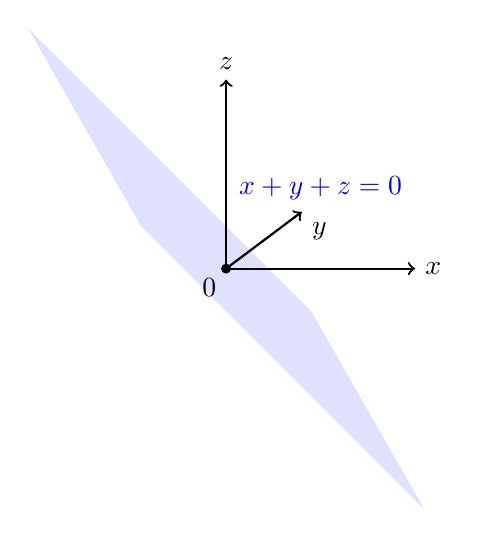
\begin{tikzpicture}[scale=1.2,
        x={(1cm,0cm)},
        y={(0.4cm,0.3cm)},
        z={(0cm,1cm)}]
        
        % Hyperplane (plane x + y + z = 0 through origin)
        \fill[blue!20, opacity=0.6] (-1.5,1.5,0) -- (1.5,1.5,-3) -- (1.5,-1.5,0) -- (-1.5,-1.5,3) -- cycle;
        
        % Coordinate axes
        \draw[->, thick] (0,0,0) -- (2,0,0) node[right] {$x$};
        \draw[->, thick] (0,0,0) -- (0,2,0) node[below right] {$y$};
        \draw[->, thick] (0,0,0) -- (0,0,2) node[above] {$z$};
        
        % Origin
        \fill (0,0,0) circle (1.5pt) node[below left] {$0$};
        
        % Label - moved to avoid overlap
        \node[blue] at (1.2,-0.5,1) {$x + y + z = 0$};
    \end{tikzpicture}
    \captionof{figure}{A hyperplane in $\bb{R}^3$: the plane $x + y + z = 0$ through the origin.}
    \end{center}
\end{example}

\begin{example}[Hyperplanes in Infinite Dimensions]
    The following are examples of hyperplanes in infinite-dimensional spaces:
    \begin{enumerate}
        \item In $K[X]$ (polynomials), let $\mathrm{ev}_0: K[X] \to K$ be evaluation at $0$:
        \[
            H = \Ker{\mathrm{ev}_0} = \Set{p \in K[X] \mid p(0) = 0}
        \]
        This is the set of polynomials with zero constant term.
        
        \item In $K^{(\bb{N})}$ (finite support sequences), define $f: K^{(\bb{N})} \to K$ by
        $f((a_n)) = \sum_{n \in \bb{N}} a_n$ (a finite sum). Then:
        \[
            H = \Ker{f} = \Set{(a_n) \in K^{(\bb{N})} \mid \sum_{n \in \bb{N}} a_n = 0}
        \]
    \end{enumerate}
\end{example}

\begin{example}[Cardinal vs Dimension: A Critical Counterexample]
\label{ex:hyperplane-counterex}
    Let $V = K[X]$ with basis $\{1, X, X^2, \ldots\}$, so $\Dim[K]{V} = \aleph_0$.
    
    Let $W = \Span[K]{\Set{X^n \mid n \geq 2}}$ (polynomials with no constant or linear term).
    Then $\Dim[K]{W} = \aleph_0$ as well.
    
    \textbf{Cardinal arithmetic suggests a hyperplane}:
    $\aleph_0 + 1 = \aleph_0 = \Dim[K]{V}$, so naively $\Dim[K]{W} + 1 = \Dim[K]{V}$.
    
    \textbf{But $W$ is NOT a hyperplane}:
    \[
        \QuotientSpace{V}{W} \cong \Span[K]{\Set{1, X}} \quad \text{has} \quad 
        \Dim[K]{\QuotientSpace{V}{W}} = 2 \neq 1
    \]
    
    \textbf{Lesson}: In infinite dimensions, the condition ``$\Dim[K]{W} + 1 = \Dim[K]{V}$'' 
    (in the cardinal sense) does NOT imply $W$ is a hyperplane. Always use the definition:
    $\Dim[K]{\QuotientSpace{V}{W}} = 1$.
\end{example}
\newpage
\section{Dual of a Linear Map}

\begin{definition}[Dual Map]
\label{def:dual-map}
    For $T: U \to V$, the \textbf{dual map} is:
    \[
        \DualMap{T}: \Dual{V} \to \Dual{U}, \quad \DualMap{T}(\varphi) = \Composition{\varphi}{T}
    \]
\end{definition}

\begin{center}
\begin{tikzcd}
    U \arrow[r, "T"] \arrow[d, "\varphi \circ T"'] & V \arrow[d, "\varphi"] \\
    K & K \arrow[l, equals]
\end{tikzcd}
\end{center}

\begin{theorem}[Functorial Properties]
\label{thm:dual-functor}
    \begin{enumerate}
        \item $\DualMap{\Identity{V}} = \Identity{\Dual{V}}$
        \item $\DualMap{(\Composition{S}{T})} = \Composition{\DualMap{T}}{\DualMap{S}}$ 
              (contravariant)
        \item $\DualMap{(aS + bT)} = a\DualMap{S} + b\DualMap{T}$
    \end{enumerate}
\end{theorem}

\begin{theorem}[Injectivity/Surjectivity Duality]
\label{thm:dual-inj-surj}
    For a linear map $T: U \to V$:
    \begin{enumerate}
        \item $\DualMap{T}$ is injective $\Leftrightarrow$ $T$ is surjective
        \item $\DualMap{T}$ is surjective $\Leftrightarrow$ $T$ is injective
    \end{enumerate}
\end{theorem}

\begin{proof}
    \textbf{(1) $\DualMap{T}$ inj $\Leftrightarrow$ $T$ surj}:
    
    ($\Leftarrow$) If $T$ surjective and $\DualMap{T}(\varphi) = \Composition{\varphi}{T} = 0$,
    then for any $v = T(u)$: $\varphi(v) = \varphi(T(u)) = 0$. Thus $\varphi = 0$.
    
    ($\Rightarrow$) If $T$ not surjective, pick $v_0 \notin \Rng{T}$, $v_0 \neq 0$.
    Extend $\{v_0\}$ to basis, define $\varphi$ with $\varphi(v_0) = 1$, $\varphi|_{\Rng{T}} = 0$.
    Then $\varphi \neq 0$ but $\DualMap{T}(\varphi) = 0$.
    
    \textbf{(2) $\DualMap{T}$ surj $\Leftrightarrow$ $T$ inj}:
    
    ($\Leftarrow$) Let $T$ be injective. For any $\psi \in \Dual{U}$, we need $\varphi \in \Dual{V}$
    with $\Composition{\varphi}{T} = \psi$.
    
    Since $T$ is injective, we can define $\varphi_0: \Rng{T} \to K$ by $\varphi_0(T(u)) = \psi(u)$.
    This is well-defined (injectivity) and linear.
    
    Choose a complement: $V = \Rng{T} \oplus W$ (by extending a basis of $\Rng{T}$).
    Define $\varphi(v) = \varphi_0(v_R)$ where $v = v_R + v_W$.
    Then $\DualMap{T}(\varphi) = \psi$.
    
    ($\Rightarrow$) If $T$ not injective, pick $u_0 \in \Ker{T}$, $u_0 \neq 0$.
    Define $\psi \in \Dual{U}$ with $\psi(u_0) = 1$ (extend $\{u_0\}$ to basis).
    
    If $\DualMap{T}(\varphi) = \psi$ for some $\varphi$, then 
    $\psi(u_0) = \varphi(T(u_0)) = \varphi(0) = 0 \neq 1$. Contradiction.
\end{proof}

\newpage
\section{Bidual and Canonical Isomorphism}

\begin{definition}[Evaluation Map]
\label{def:evaluation}
    The \textbf{evaluation map} is:
    \[
        \eta_V: V \to \Dual{\Dual{V}}, \quad \eta_V(v)(\varphi) = \varphi(v)
    \]
\end{definition}

\begin{theorem}[{$\eta_V$ is Always Injective}]
\label{thm:eta-injective}
    $\Ker{\eta_V} = \Set{0}$ for any $V$.
\end{theorem}

\begin{proof}
    If $\eta_V(v) = 0$ and $v \neq 0$, extend $\{v\}$ to basis, define $\varphi_0(v) = 1$.
    Then $\varphi_0(v) = 1 \neq 0 = \eta_V(v)(\varphi_0)$. Contradiction.
\end{proof}

\begin{theorem}[Canonical Isomorphism]
\label{thm:canonical-iso}
    $\eta_V: V \xrightarrow{\cong} \Dual{\Dual{V}}$ iff $\Dim[K]{V} \in \bb{N}$.
\end{theorem}

\begin{proof}
    ($\Leftarrow$) If $\Dim[K]{V} = n \in \bb{N}$, then 
    $\Dim[K]{\Dual{\Dual{V}}} = \Dim[K]{\Dual{V}} = n$.
    Injective + equal dimensions $\Rightarrow$ isomorphism.
    
    ($\Rightarrow$) If infinite-dim, $\Dim[K]{\Dual{\Dual{V}}} > \Dim[K]{\Dual{V}} > \Dim[K]{V}$.
    Cannot be surjective.
\end{proof}

\begin{remark}[Canonicity]
\label{rem:canonical}
    $\eta_V$ is \textbf{canonical}: no basis choice needed.
    
    \textbf{Naturality}: For $T: U \to V$, the following commutes:
    \begin{center}
    \begin{tikzcd}
        U \arrow[r, "\eta_U"] \arrow[d, "T"'] & \Dual{\Dual{U}} \arrow[d, "\DualMap{\DualMap{T}}"] \\
        V \arrow[r, "\eta_V"'] & \Dual{\Dual{V}}
    \end{tikzcd}
    \end{center}
    
    Proof: $(\DualMap{\DualMap{T}}(\eta_U(u)))(\psi) = \eta_U(u)(\DualMap{T}(\psi)) = 
    (\Composition{\psi}{T})(u) = \psi(T(u)) = \eta_V(T(u))(\psi)$.
\end{remark}
